% !TeX root = hw_1-koncni_avtomati.tex
\documentclass{article}

\usepackage{graphicx}
\usepackage{tikz}
\usepackage{parskip}
\usetikzlibrary {arrows.meta,automata,positioning}
\title{Algoritmi v bioinformatiki - 1. Domača naloga}
\author{Jan Panjan}
\date{\today}

\begin{document}

\tikzset{
node distance=2.6cm, % specifies the minimum distance between two nodes. Change if necessary.
every state/.style={thick, fill=gray!10}, % sets the properties for each ’state’ node
->, % makes the edges directed
>={Stealth} % make arrow heads bold
}

\maketitle
\newpage

\begin{enumerate}
	\item \textit{Konstruirajte deterministični končni avtomat, ki v mRNK materialu prepozna
		zaključne kodone.}
		\begin{enumerate}
			\item Grafično:

				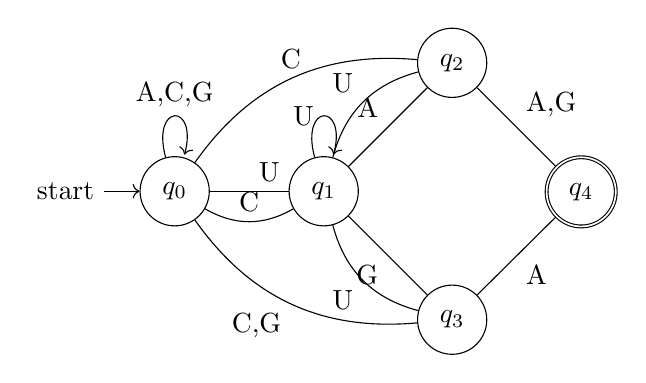
\begin{tikzpicture}
					\node[state, initial]   (q0)                     {$q_0$};
					\node[state] 			(q1) [right=of q0]       {$q_1$};
					\node[state] 	        (q2) [above right=of q1] {$q_2$};
					\node[state] 		    (q3) [below right=of q1] {$q_3$};
					\node[state, accepting] (q4) [below right=of q2] {$q_4$};

					\draw (q0) edge[loop above] node{A,C,G} (q0)
					 (q0) edge[above right] node{U} (q1)

					 (q1) edge[above, bend left] node{C} (q0)
					 (q1) edge[above left] node{A} (q2)
					 (q1) edge[below left] node{G} (q3)
					 (q1) edge[loop above, left] node{U} (q1)

					 (q2) edge[above left, bend right] node{U} (q1)
					 (q2) edge[above right] node{A,G} (q4)
					 (q2) edge[above, bend right] node{C} (q0)

					 (q3) edge[below left, bend left] node{U} (q1)
					 (q3) edge[bend left, below left] node{C,G} (q0)
					 (q3) edge[below right] node{A} (q4);
				\end{tikzpicture}

			\item S formalnim opisom peterike $\left[ \Sigma, Q, q_0, F, \delta \right]$:

				\begin{itemize}
					\item $\Sigma = \{ A, U, C, G \}$
					\item $Q = \{ q_1, q_2, q_3, q_4 \}$
					\item $q_0 = q_0$
					\item $F = \{ q_4 \}$
					\item stanja so pisana samo s številko in pot ki pripelje do
						končnega stanja je označena z rdečo barvo, da je bolj
						berljivo.

						\begin{tabular}{|c||c|c|c|c|}
							\hline
							$\delta$ & A & U & C & G \\
							\hline \hline
							0 & 0 & \textcolor{red}{1} & 0 & 0 \\
							\hline
							1 & \textcolor{red}{2} & 1 & 0 & \textcolor{red}{3} \\
							\hline
							2 & \textcolor{red}{4} & 1 & 0 & \textcolor{red}{4} \\
							\hline
							3 & \textcolor{red}{4} & 1 & 0 & 0 \\
							\hline
							4 & / & / & / & / \\
							\hline
						\end{tabular}
				\end{itemize}
		\end{enumerate}

		\newpage

	\item \textit{Kako se rešitev 1. naloge spremeni, če želimo s pomočjo končnega
			avtomata poiskati vse pojavitve zaključnih kodonov? Zapišite algoritem
			in ponazorite njegovo delovanje na delu mRNK AUAUAAUGCUUGA. Koliko
		zaključnih kodonov vsebuje dani mRNK?}

		Njegovo končno stanje se spremeni, tako da ponovno začne iskati vzorec, ko
		pride enkrat do
		končnega stanja. To je vidno grafično kot povezava od $q_4$ do $q_0$ in
		spremenjene vrednosti v zadnji vrstici $\delta-$tabele.

		\begin{enumerate}
			\item Grafično:

				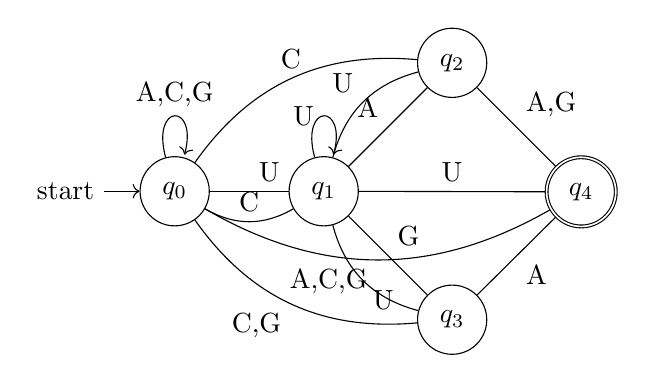
\begin{tikzpicture}
					\node[state, initial]   (q0)                     {$q_0$};
					\node[state] 			(q1) [right=of q0]       {$q_1$};
					\node[state] 	        (q2) [above right=of q1] {$q_2$};
					\node[state] 		    (q3) [below right=of q1] {$q_3$};
					\node[state, accepting] (q4) [below right=of q2] {$q_4$};

					\draw (q0) edge[loop above] node{A,C,G} (q0)
					 (q0) edge[above right] node{U} (q1)

					 (q1) edge[above, bend left] node{C} (q0)
					 (q1) edge[above left] node{A} (q2)
					 (q1) edge[above right] node{G} (q3)
					 (q1) edge[loop above, left] node{U} (q1)

					 (q2) edge[above left, bend right] node{U} (q1)
					 (q2) edge[above right] node{A,G} (q4)
					 (q2) edge[above, bend right] node{C} (q0)

					 (q3) edge[below right, bend left] node{U} (q1)
					 (q3) edge[bend left, below left] node{C,G} (q0)
					 (q3) edge[below right] node{A} (q4)

					 (q4) edge[above] node{U} (q1)
					 (q4) edge[bend left, below left] node{A,C,G} (q0);
				\end{tikzpicture}

			\item S formalnim opisom peterike $\left[ \Sigma, Q, q_0, F, \delta \right]$:

				\begin{itemize}
					\item $\Sigma = \{ A, U, C, G \}$
					\item $Q = \{ q_1, q_2, q_3, q_4 \}$
					\item $q_0 = q_0$
					\item $F = \{ q_4 \}$
					\item \begin{tabular}{|c||c|c|c|c|}
							\hline
							$\delta$ & A & U & C & G \\
							\hline \hline
							0 & 0 & \textcolor{red}{1} & 0 & 0 \\
							\hline
							1 & \textcolor{red}{2} & 1 & 0 & \textcolor{red}{3} \\
							\hline
							2 & \textcolor{red}{4} & 1 & 0 & \textcolor{red}{4} \\
							\hline
							3 & \textcolor{red}{4} & 1 & 0 & 0 \\
							\hline
							4 & 0 & 1 & 0 & 0 \\
							\hline
						\end{tabular}
				\end{itemize}
		\end{enumerate}

		\textbf{Algoritem za iskanje STOP kodonov v mRNA vzorcu:} algoritem za izgradnjo
		$\delta-$tabele smo podali na vajah in ga ne bom ponovno napisal.
		Predpostavljam torej, da je tabela za naš končni avtomat že izgrajena.
		Iskanje vzorca v besedilu AUAUAAUGCUUGA poteka tako:

 		kaj je mišljeno kot algoritem tu..?

		Dani vzorec mRNA vsebuje dva stop kodona: AUA\textcolor{red}{UAA}UGCU\textcolor{red}{UGA}

	\item \textit{Konstruirajte determinističen končni avtomat za naslednji
			nedeterminističen končni avtomat.}

		Deterministični končni avtomat iz nedeterminističnega izgradimo s pomočjo
		$\delta-$tabele tako da zapišemo vse neprazne podmnožice stanj. Za stanje
		npr. $1,2$ naredimo unijo sledečih stanj za $a$ in $b$, t.j $1,2,3$ in $2$., t.j $1,2,3$ in $2$.
		Da se izognemo pisanju nepotrebnih stanj, naredimo tabelo samo za dosegljiva
		stanja.

		\textbf{Nedeterminističen končni avtomat:}

		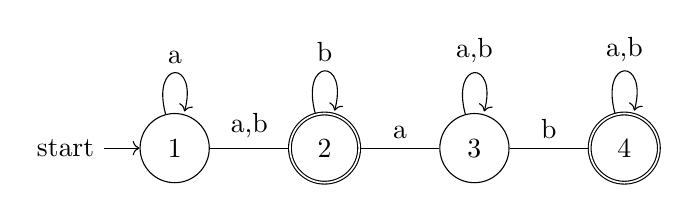
\begin{tikzpicture}
			\node[state, initial]   (q1)               {$1$};
			\node[state, accepting]	(q2) [right=of q1] {$2$};
			\node[state] 	        (q3) [right=of q2] {$3$};
			\node[state, accepting] (q4) [right=of q3] {$4$};

			\draw (q1) edge[loop above] node{a} (q1)
				(q1) edge[above] node{a,b} (q2)
				(q2) edge[loop above] node{b} (q2)
				(q2) edge[above] node{a} (q3)
				(q3) edge[loop above] node{a,b} (q3)
				(q3) edge[above] node{b} (q4)
				(q4) edge[loop above] node{a,b} (q4);
		\end{tikzpicture}

		\textbf{$\delta-$tabela:}

		\begin{tabular}{|c||c|c|}
			\hline
			$\delta$ & a & b \\
			\hline\hline
			1 & 1,2 & 2 \\
			\hline
			2 & 3 & 2 \\
			\hline
			3 & 3 & 3,4 \\
			\hline
			4 & 4 & 4 \\
			\hline
			1,2 & 1,2,3 & 2 \\
			\hline
			3,4 & 3,4 & 3,4 \\
			\hline
			1,2,3 & 1,2,3 & 2,3,4 \\
			\hline
			2,3,4 & 3,4 & 2,3,4 \\
			\hline
		\end{tabular}

		Končna stanja sta $2$ in $4$, zato bo imel novi končni avtomat za končna
		stanja vsa stanja, ki vsebujejo tako $2$ ali $4$.

		Zgodi se, da stanje $4$ odpade, saj nobeno stanje ne vodi vanj.

		\textbf{Determinističen končni avtomat:}

		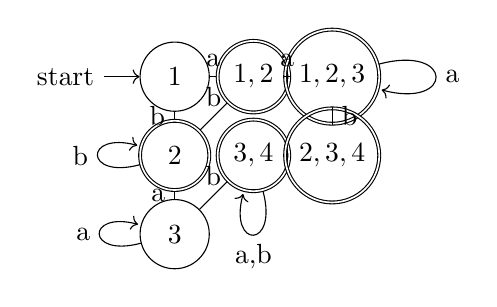
\begin{tikzpicture}
			\node[state, initial] (1) {$1$};
			\node[state, accepting] (2) [below of=1] {$2$};
			\node[state] (3) [below of=2] {$3$};
			\node[state, accepting] (12) [right of=1] {$1,2$};
			\node[state, accepting] (123) [right of=12] {$1,2,3$};
			\node[state, accepting] (34) [below of=12] {$3,4$};
			\node[state, accepting] (234) [below of=123] {$2,3,4$};

			\draw (1) edge[left] node{b} (2)
				(1) edge[above] node{a} (12)
				(12) edge[above] node{b} (2)
				(12) edge[above] node{a} (123)
				(123) edge[loop right] node{a} (123)
				(123) edge[right] node{b} (234)
				(2) edge[loop left] node{b} (2)
				(2) edge[left] node{a} (3)
				(3) edge[loop left] node{a} (3)
				(3) edge[above] node{b} (34)
				(34) edge[loop below] node{a,b} (34);
		\end{tikzpicture}

	\item haha

\end{enumerate}

\end{document}
